\chapter{Introduction}
\label{cha:Introduction}

Autonomous Vehicles, or AVs, used to exist solely in science fiction. In 1953, Isaac Asimov wrote \emph{Sally} \citep{Asimov1953} and in 1982, \emph{Knight Rider} introduced KITT \citep{Kitt1982}. Today, AVs can be found on roads around the world. Alphabet's WAYMO is gaining traction, with cars being tested in four different US states \citep{Waymo2016}. Tesla have deployed their beta Autopilot system into all of their vehicles produced since September 2014 \citep{TeslaAutoPressKit}. The system has been both hailed for saving lives and blamed for ending them \citep{TeslaHospital} \citep{TeslaUnderInvestigation}.

All of the AV systems currently running on public roads are designed to work alongside human driven vehicles, limiting their benefits. In order to truly embrace AVs, we need to design systems which assume every vehicle on the road is automated. The advantages of these systems are numerous, but the most important benefit is safety.

AVs would be able to react to incidents much more quickly than a human driver could. A driver's `thinking distance' often determines whether someone survives an accident or not. This distance can be greatly increased if the driver of the vehicle is under the influence of alcohol or narcotics. An AV would be able to react to accidents much more quickly than a human, reducing the thinking distance and improving road safety. Figure \ref{fig:StoppingDistances} shows the impact thinking distance can have on the overall stopping distance of vehicle.

\begin{figure}[htb]
\centerline{
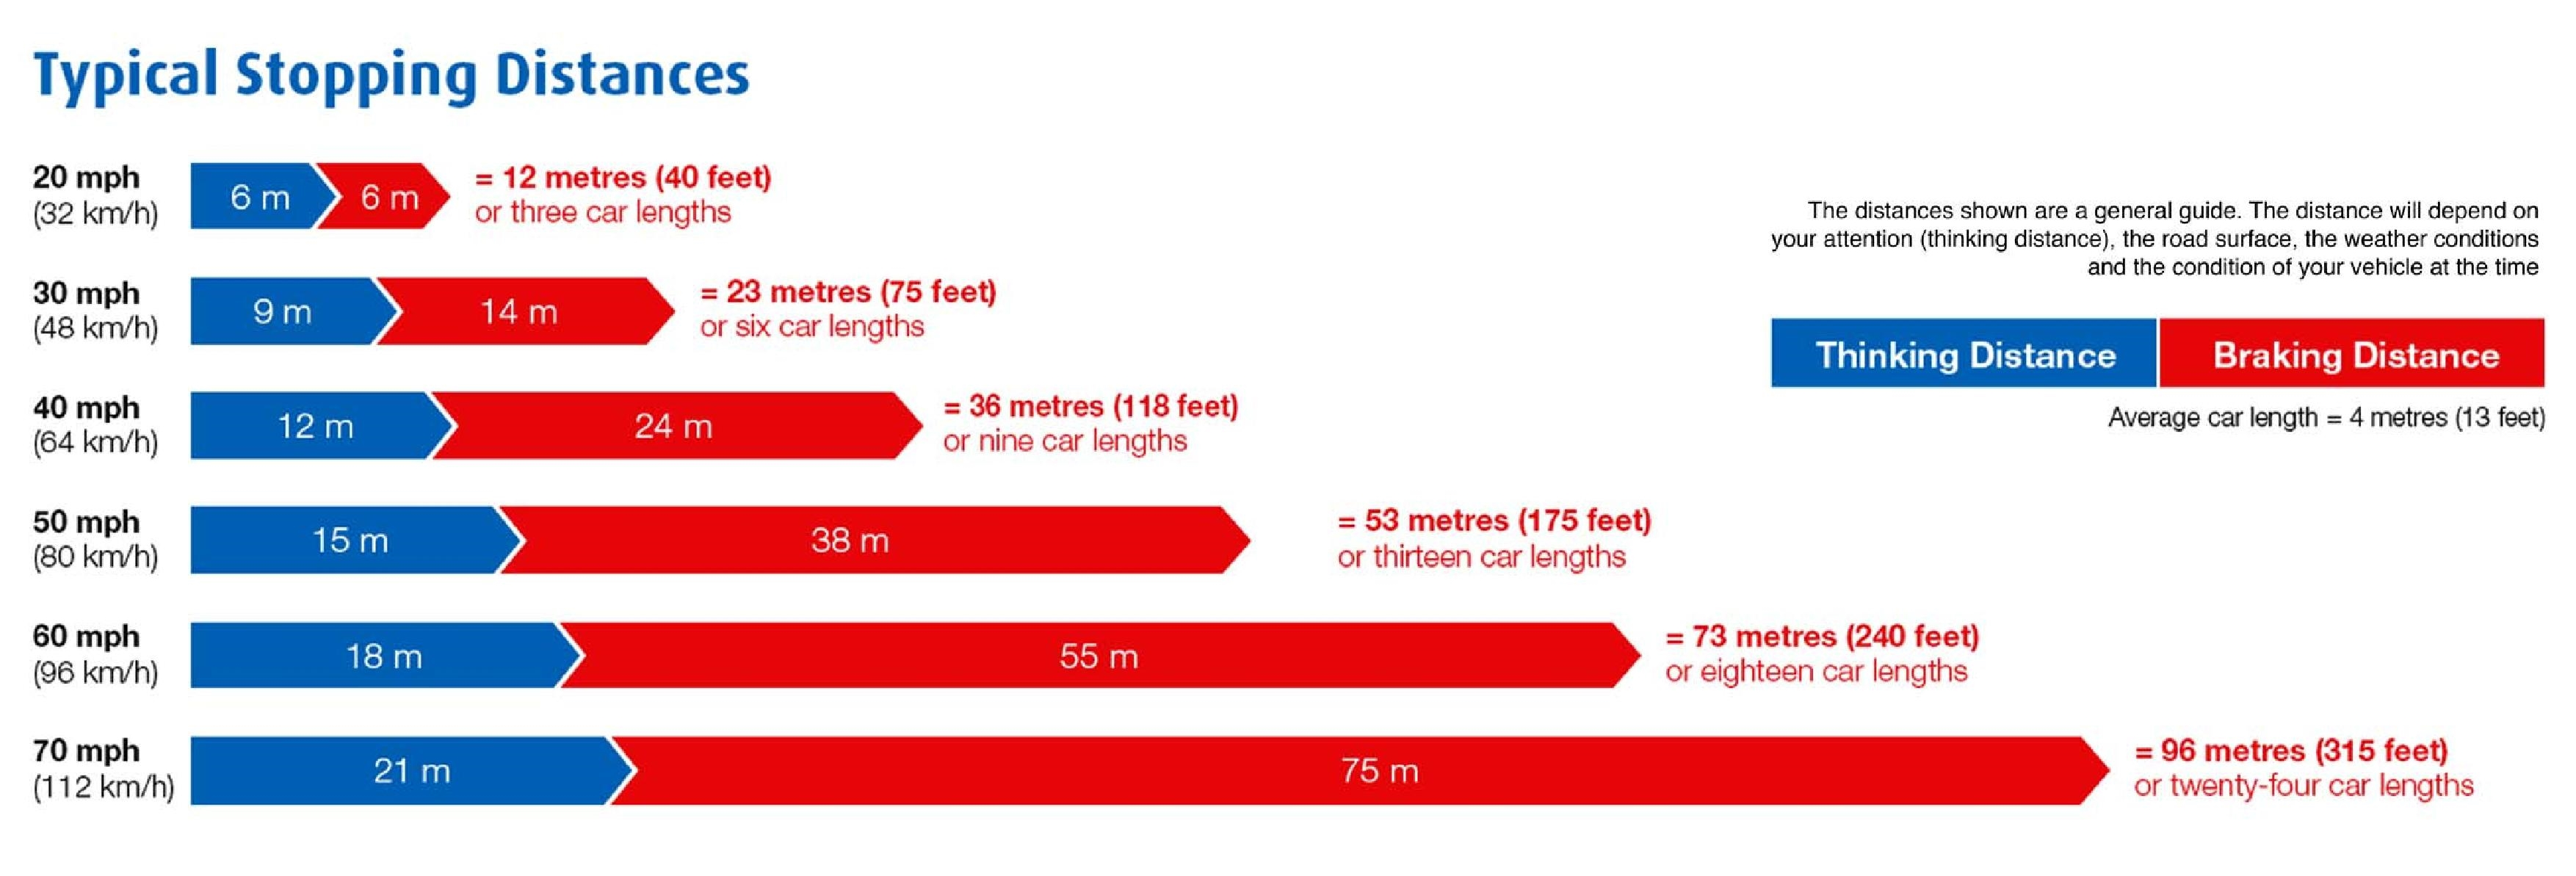
\includegraphics[width=15cm]{introduction/stoppingDistances.jpg}
}
\caption{Diagram from Rule 126 in the UK Highway Code \citep{StoppingDistances}}
\label{fig:StoppingDistances}
\end{figure}

Another benefit of AVs is efficiency. Research suggests that by implementing fuel conserving driving strategies, AVs could be up to 10\% more fuel efficient than current EPA fuel economy test results \citep{Mersky2016}. Fuel efficient vehicles are becoming increasingly important, with landmark climate change deals such as `The Paris Agreement' introducing limits on greenhouse gas emissions globally \citep{Paris2016}. The introduction of electric vehicles into the car market is also an important factor to consider, as the driving range of such vehicles has still not managed to match that of their gasoline counterparts. Introducing efficient driving strategies through AVs could help bring electric vehicle range up to par.

Congestion contributes to fuel waste in quite a large way. In 2014, the US wasted an estimated 3.1 billion gallons (11.7 billion litres) of fuel due to congestion \citep{Schrank2015}. Automated driving strategies, in situations such as lane changes, could reduce congestion and improve efficiency. Dangerous lane changes don't even have to result in a crash to cause delays. If a car brakes due to a dangerous merge, it can cause a ripple effect, creating congestion. This ripple effect is known as a `traffic shock' \citep{Daganzo1994}.

As well as more quantifiable benefits, AVs could also provide a level of comfort not currently available today. In a world where AVs are commonplace, it is not hard to imagine people working, reading or relaxing in their car instead of focusing on driving. 

However, today there are still a number of concerns surrounding AVs, one major issue being the reliability of the systems governing the vehicle. Systems need to be responsive and accurate. They cannot afford to fail in such safety critical environments. Today, concerns over Tesla's Autopilot system are impacting the image of the company, and the system isn't even out of beta yet \citep{TeslaCriticised}. 

In order to address these concerns safely, we can create simulations which test the reliability of autonomous systems. Researchers at the University of Texas set up the Autonomous Intersection Management (AIM) project, which aims to "create a scalable, safe, and efficient multi-agent framework for managing Autonomous Vehicles at intersections" \citep{AIMProject}. The team managed to apply their simulator tested intersection software in a mixed reality test, using a real life AV \citep{Quinlan2010}. This demonstrates how vital simulators are when testing safety critical systems.

The motivation for the AIM system was to reduce congestion at intersections. Similarly to intersections, lane merges can be significant sources of congestion. AVs will need to be able to deal with various lane merge situations if they are to become effective alternatives to manual vehicles. This project aims to develop a simulator that can effectively filter traffic through a lane merge. This simulator will be based on the AIM simulator codebase, which will also be considered for future AV projects if it can be adapted effectively. Using this simulator we aimed to compare different merge schemes, particularly looking at the effectiveness of decentralised systems against centralised systems. We also aimed to analyse how different merge conditions impact the performance of a merge system.

This project makes a number of assumptions. Firstly we assume that the sensors resolving the positions of the vehicle and it's surrounding obstacles are perfectly accurate. We also assume that all vehicles can reliably communicate with each other and with roadside infrastructure. These assumptions ignore existing areas of research which are not considered in this paper.

Chapter \ref{cha:Literature Review} examines existing work with merging AVs and compares centralised approaches to decentralised approaches. Chapter \ref{cha:Problem Analysis} takes a deeper look at the issues surrounding lane merges and the different types of lane merges that can be found on the roads today. Chapter \ref{cha:Design} examines different approaches to the merge problem and their advantages and disadvantages. Chapter \ref{cha:Implementation} details some of the problems encountered whilst implementing the merge approaches, and the reasons for some of the workarounds implemented. Chapter \ref{cha:Results} analyses the performance of the Queue Merge Management system and compares it to a modified AIM implementation.